\documentclass[11pt]{article}
% \usepackage[margin=1in]{geometry}
\usepackage{titlesec}
\titlespacing*{\section}{0pt}{0.5\baselineskip}{0.4\baselineskip}
\usepackage{enumerate}
\usepackage{cite}
\usepackage{forest}
\usepackage[margin=1in]{geometry}
\usepackage{mathtools}
\usepackage{amsmath}
\usepackage{amssymb}
\usepackage{gensymb}
\usepackage{hyperref}
\usepackage{floatrow}
\usepackage{subcaption}
\usepackage{caption}
\usepackage{float}
\restylefloat*{figure}
\floatsetup[table]{capposition=top}
\usepackage{filecontents}
%\usepackage{biblatex}
\usepackage[T1]{fontenc}
% for proper encoding
\usepackage[utf8]{inputenc}
% enhanced font Latin Modern
\usepackage{lmodern}
% multi-language support
\usepackage[english]{babel}
% for inline and display quotations.
\usepackage[autostyle]{csquotes}
\usepackage{url}
% set the default 4 inches margin to be 1 inch
\usepackage{fullpage}
%\setlength{\parindent}{em}
\setlength{\parskip}{0.5em}
\renewcommand{\baselinestretch}{1}
%\usepackage[demo]{graphicx}
%opening

\title{CSCI 491/591 P6}
\date{April 28, 2016}
\author{Group 4\\Chenglin Fan, Jici Huang,
Angelica Davis, and Peng Zou}
\begin{document}
\maketitle
\vspace{-0.4 in}
%P3: Data visualization (20 points). Now that you have chosen a data
%set, part of research in data analysis is presenting the data in a way that
%is understandable to a reader (or reviewer). This is best done through
%figures that capture essential features of your data set. These figures can
%be projections of the data set into the plane, histograms measuring some
%quantity computed over your data, a figure illustrating from where your
%data was sampled, etc. [Deliverable: five figures, with captions and labels].\\
\noindent


  In this project our group is exploring a data sets comprised of GPS trajectories collected from taxi `trips' around various major cities across the globe, such as Athens in Greece, Berlin in Germany, Chicago in US, and Beijing in China. In the award winning paper, ``Efficient Map Reconstruction and Augmentation via Topological Methods''~\cite{Wang15}, the GPS trajectories of major cities were processed using two critical topological concepts, persistence~\cite{edelsbrunner2008persistent} and Morse Theory~\cite{milnor1963morse}, in order to construct an accurate image of the road networks of these major cities. The ultimate goal of our project is to deeply understand the topological concepts and techniques used in the paper to analyze GPS trajectories, and to add these data processing techniques to our skill sets, since they have been shown to be effective against a variety of noise that are common to  practical and experimental data.
  \par Our group selected the GPS trajectories data set of Berlin among several others, that we have explored in the project. The Data Set Selection section provides information about where the data set is from, and several reasons why the particular data set was selected. 
  
  
In the second part, we show the  several steps in the map reconstruction process, which includes the pre-processing of trajectory data, the density field calculation, ridge extraction and  simplification of the road network.
Then, we illustrate the visualization of results we got in this project, including the visualization of trajectory data, the resulting map from extracting the ridge of the terrain and the map after persistence simplification.
Finally, we give the conclusion and possible improvements to work on in the future.

\section*{Data Set Selection}
\par
In recent years, the amount of Volunteered Geographic Information (VGI) data that is publicly available has grown very fast, and the computational map construction from these GPS trajectories has attracted great attention.~\cite{Wang15} The data set selected for this project was the VGI trajectory data of Berlin, Germany. The items below discuss why the Berlin trajectory data set was chosen.%Our group believes that the trajectory data of Berlin is a suitable representative data set based on several reasons below.
%In P1, we went through all data sets provided by Map Construction Portal and we decided to investigate trajectory data of the tracks in Berlin, large. 
% It is a suitable representative data set because the size of the trajectory data is about midway between Chicago and Athens.
\par
First, GPS trajectory information has many very practical uses, therefore there is much value in knowing how to process and analyze data sets of this type. 
\par
Second, VGI data sets tend to be massive in size. The data set selected for Berlin contains a moderate number of trips and GPS samples per trip when compared to data sets of other cities. This makes it a good candidate for efficient processing given the time constraint, since the input data set size has a significant impact on the running time of the algorithm. Additionally, it contains enough densely overlapping trip data for the algorithm to produce a road network estimation with a degree of confidence (this will be explained more thoroughly in the steps section).%The size of the Berlin data set is neither too large for efficient reconstruction, nor too small for evaluating the effectiveness of the algorithm.  %Thus, the trajectory data of Berlin can well represent the GPS data.
\par
Third, the data sets are all open source. The data set is accessible via the Internet, and can be downloaded from the open source website conveniently~\cite{link}, and many researchers~\cite{Wang15} use this data for research, hence it is easy to compare between the results of our experiment and the results of other people's work.
%\par
%Last but not least, the quality of the data sets are guaranteed. The data set has a comparable characteristic since the data set contains overlapping trajectories as well as noisy trajectories (either due to noisy trajectories or lack of sampling uniformity).  % This doesn't really make any sense
% Data set choice (8 points). You must select an interesting data set
% that you will investigate in this project. The data set can be real (GPS trajectories,
% Four-square check-ins, gene expressions, March madness brackets,
% baseball statistics, 3D objects, movie scripts, etc.), or it can be theoretical
% (flip graphs, the space of image patches, etc.). [Deliverable: one-to-two page write-up].

\section*{Details of the Data}
\par % agreement: "was" is singular, trajectories is plural and "English" can be tricky!
The data set of Berlin GPS trajectories was downloaded from the Map Construction Portal~\cite{link}. The GPS trajectories of Berlin contain the trajectory data of taxi trips in Berlin. A trip is a collection of discretely sampled GPS trajectories that describe one path traveled through the city over some time period. The trajectory data has more than 27,000 trips in .txt format. 
\par
Each trip file consists of a list of trajectory data represented by an x-coordinate, y-coordinate and time stamp. Table \ref{table:questions} provides a partial sample of a trip file taken from the trajectory data of Berlin.
\begin{table}[h!]
\begin{center}
\begin{tabular}{ |c |c| c| }
\hline
  time-stamp & x & y    \\ \hline
  2585542.00 & 393742.586772 & 5821049.184616    \\ \hline
  2585604.00 & 393747.949682 & 5821296.284551  \\  \hline
  2585677.00 & 393883.091662 & 5821448.203015  \\ \hline
  2585738.00 & 393759.343945 & 5821821.259046  \\ \hline
\end{tabular}
\end{center}
\caption{An excerpt of trajectory data of Berlin}
\label{table:questions}
\end{table}





\begin{figure}[H]
  \caption{A visualization of discretely sampled points of the trajectory data of Berlin, as they are collected by taxi drivers' GPS systems. The points are actually physically far apart. We set the scale to $10^5$ for $x$ axis and $10^6$ for $y$ axis, which enable us to see the big picture of the points with the scale.}
  \centering
 \includegraphics[scale=0.5]{RawVerticesCircle.eps} 
\end{figure}

\section*{Steps to Reconstruct the Map}
\par
Our group uses the map reconstruction algorithm~\cite{Wang15} to estimate the Road Network, which includes converting input trajectories to a density map, and  extracting the ridge of the 
density map; the  steps are as follows.   

\par
 \textbf{Density Field Construction:} Discretize the region of city into a
grid where each grid cell has side-length $r$. Each input trajectories is a sequence of discrete  sampled points,  let P = $\{p_1,p_2,p_3,...,p_n\}$ be the collection of discrete sampled points
from the trajectories. Compute the density $\rho(g)$ for  each grid point $g$ ($g_x,g_y$) based on the density function in paper~\cite{Wang15}.
\par
\textbf{Ridge Extraction:} The set of points $\{(g_x,g_y,\rho(g)) \}$ in $\mathbb{R}^3$ is a discrete terrain, compute the saddle points in the terrain, where saddle point of terrain is a stationary point but not an extreme point. Then we compute the 
manifold $S(p)$ for each saddle point $p$, where $S(p)$  is the collection
of points of the terrain such that for each point $q$ in $S(p)$, there is a  monotone  descending path from $q$ to $p$, and $S(p)$ is usually composed of  discrete curves (each of them is from a local maximum point to $p$ ).
\par
\textbf{Persistence Simplification:} The persistence is used to measure the scale or
resolution of a topological feature. Compute the persistence~\cite{edelsbrunner2008persistent} for each manifold $S(p)$ (whose projection is a piece of  road), the persistence value is equal the difference between the density of  local maximal point and the density of saddle point. We remove all the  manifolds
(unimportant roads) whose persistence is smaller than a given value. At last we project the remaining manifolds onto the plane, and obtain the road network of city.



\section*{Experimental Results}


\subsection*{Trajectory Data  Visualization}
Each trip of the trajectory data is composed of a series of discrete points. Figure $1$ shows the discrete points of the trips in Berlin. We can barely figure out the main roads from the spread out points in Figure $1$, nor in the map of the city. In Figure $1$, some regions have higher density of the discrete points while other parts have lower density of the discrete points. But even the higher density regions are not connected to each other, it is impossible to get the map of the city directly without further processing. 
\subsection*{Density Field Visualization}
In map reconstruction, the first step is density calculation.  In P2,  we gave the detail to compute the density $\rho(g)$ for each grid point $g$ based on the density function~\cite{Wang15}. We set the grid size be $10m$, and the parameter $t$ (roughly indicates the noise level) be $\sqrt{t}=20 m$. Figure $2$ is the visualization of the density field after calculation, the very high density regions are colored in green or blue, the high level density regions are colored in red, and the low density regions are colored in dark red. The underlying main road networks are much clearer based on the density field map. 

\begin{figure*}[t!]
    \centering
    \begin{subfigure}[t]{0.5\textwidth}
        \centering
        \includegraphics[height=2.9in]{densityMapAerialfig.eps}
        \caption{The demonstrates of the density field in two-dimension.}
    \end{subfigure}%
    ~
    \begin{subfigure}[t]{0.5\textwidth}
        \centering
        \includegraphics[height=2.9in]{densityMap.eps}
        \caption{The demonstration of the density field in three-dimension.}
    \end{subfigure}
    \caption{The figure demonstrates the density distribution of trajectories. It is the visualization of the density field after calculation, the very high density regions are colored in green or blue, the high level density regions are colored in red, and the low density regions are colored in dark red. The underlying main road networks are much clearer based on the density field map.}
\end{figure*}

\subsection*{Ridge Extraction}
The detail of ridge extraction is given in P$2$. The motivation of ridge extraction is to obtain the skeleton of the map for the following reasons.\\
First, even the high density regions in density filed map has width  much larger than the real network of city. Hence, the directly use of high density regions is not suitable to obtain the map. Second, it
can detect roads with few trajectories passing them even when they
are next to heavily populated roads, which is usually
challenging. Last but not least, it is convenient for further simplification on the current map later.

Figure $3$ shows the map obtained by extracting the ridge (we use a little extra operation to add the connection in junction).
 \begin{figure}[H]
  \caption{The map is obtained by extracting the ridge of density terrain and project it in the plane (we use a little extra operation to add the connection in junction). You can get detailed information of roads in the city.}
  \centering 
 \includegraphics[scale=0.6]{ex1.eps} 
\end{figure}

\subsection*{Persistence Simplification}
\begin{figure}[h!]
  \caption{The simplification of the map with by removing all unimportant roads whose persistence are not greater than a given value 0.05, and you can find the outline of the city (main roads in the city). We found out from the figure that Berlin has smoothly distributed roads across the city.} 
  \centering
 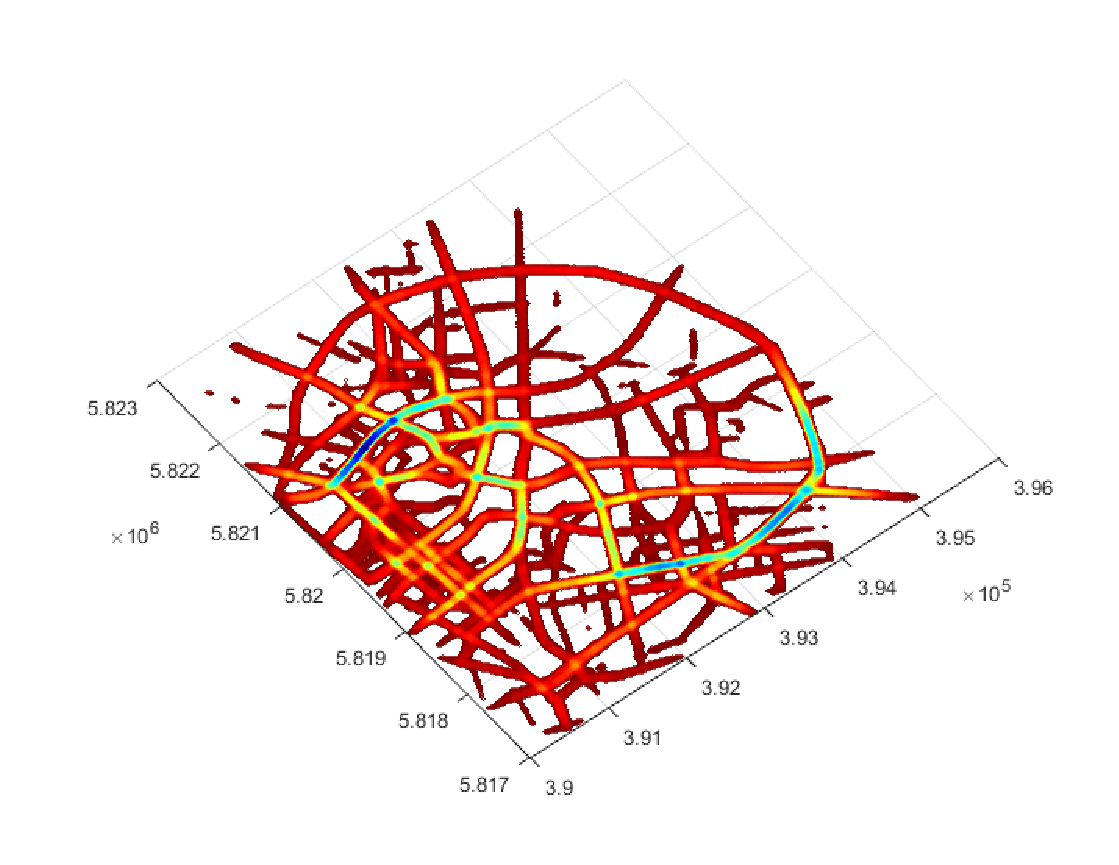
\includegraphics[scale=0.6]{p1.eps} 
\end{figure}
We compute the persistence~\cite{edelsbrunner2008persistent} for each road, and remove all unimportant roads whose persistence are not greater than a given value. By applying the persistence, we obtain the  road network after simplification. Figure $4$ shows the important roads after simplification. It also shows the connectivity of the map is decreased after simplification. Our group will further improve the performance of simplification.
\section*{Conclusion and Future Work}
\par
The project that our group is working on is interesting and fascinating. All members are excited to explore the GPS data by the applications of GPS that are affecting every aspect of modern life.    We investigated the background of reconstructing data from trajectory data, and implemented  the method in paper~\cite{Wang15}, and illustrated the results we got by now.


The  density function in paper~\cite{Wang15} can be used to deal with noise.
Two important concepts used in this project are discrete morse theory and persistence.  Morse theory enables one to analyze the topology of a manifold, by extracting the ridge. Then, we can capture the skeleton of the density terrain of grid points, which has several advantages, one of which is to obtain road with equal width, the other is to detect the roads with low density.   The  purpose of persistence is to measure  the scale or
resolution of a topological feature. In this project, we used the persistence to measure the importance of curves (whose projection be roads of map). We removed the roads whose persistence is less or equal than a given value, which make the map much clearer after simplification.    




There are several aspects can be improved in this project in the future. First, the visualization of map can be improved by using some plug-in components of Java, we print the map using java code directly by now, and it is not a vector map.  What is more, we can compare the map we got with the google map in the future.  The persistence is not the only factor in determining the importance of roads, we can combine the other factors like the length of road, and the density of road \textit{et al.} together, which can improve the performance of the map after simplification.
It would also be interesting to explore how to support more functionalities
based on the current framework, such as returning a potential
path for an input query region.







\bibliography{references}{}
\bibliographystyle{plain}
\end{document}
